\chapter{Lichtspectra en de boodschap van het licht}\label{ch:g10:light-spectra}

Een bundel sterrenlicht is het enige monster van een ster dat we ooit in
handen zullen krijgen, en het blijkt een royaal monster te zijn. Spreid
de bundel uit tot zijn \omterm{def:g10:light-spectra:white}{spectrum} --- een glazen prisma doet het, een
gordijn van regendruppels doet het --- en het licht wordt een boodschap:
een doorlopende regenboog als achtergrond verraadt de temperatuur van de
ster, en een streepjescode van fijne lijnen spelt, element voor element,
waaruit de ster bestaat. Dit hoofdstuk leert beide delen van die
boodschap lezen --- eerst op laboratoriumlampen, daarna op de Zon.

\section{Wit licht en zijn spectrum}

\begin{definition}[Ontleding van wit licht]\label{def:g10:light-spectra:white}
Wanneer een smalle bundel zonlicht een glazen prisma doorkruist, komt hij
er uitgespreid uit als een doorlopende band van kleuren, van rood tot
violet. Die band is het \emph{spectrum}\index{spectrum} van het licht.
Licht dat alle zichtbare kleuren bevat, zoals zonlicht of het licht van
een gewone gloeilamp, heet \emph{wit licht}\index{wit licht}. Licht van
één zuivere kleur, dat geen enkel prisma nog verder kan splitsen, is
\emph{monochromatisch}\index{monochromatisch licht} (een laserbundel
bijvoorbeeld); een mengsel van meerdere kleuren is
\emph{polychromatisch}\index{polychromatisch licht}. Een instrument dat
de ontleding uitvoert en de samenstelling van een licht afleest, is een
\emph{spectroscoop}\index{spectroscoop}.
\end{definition}

\begin{omfigure}
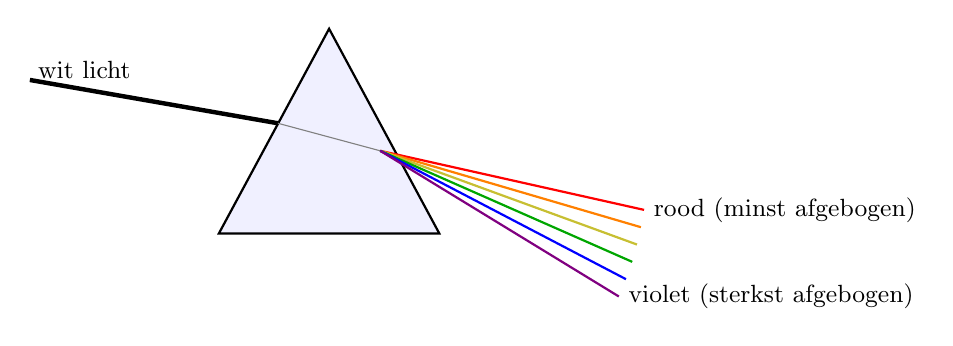
\begin{tikzpicture}[scale=1.0, font=\small]
  \draw[thick, fill=blue!6] (0,0) -- (1.4,2.6) -- (2.8,0) -- cycle;
  \draw[line width=1.6pt] (-2.4,1.95) -- (0.75,1.4)
    node[pos=0.22, above] {wit licht};
  \draw[gray] (0.75,1.4) -- (2.05,1.05);
  \draw[red, thick]              (2.05,1.05) -- (5.4,0.30);
  \draw[orange, thick]           (2.05,1.05) -- (5.36,0.08);
  \draw[yellow!75!black, thick]  (2.05,1.05) -- (5.31,-0.14);
  \draw[green!65!black, thick]   (2.05,1.05) -- (5.25,-0.36);
  \draw[blue, thick]             (2.05,1.05) -- (5.17,-0.58);
  \draw[violet, thick]           (2.05,1.05) -- (5.08,-0.80);
  \node[right] at (5.4,0.30)  {rood (minst afgebogen)};
  \node[right] at (5.08,-0.80) {violet (sterkst afgebogen)};
\end{tikzpicture}

{\small Een prisma waaiert een bundel \omterm{def:g10:light-spectra:white}{wit licht} uit tot zijn \omterm{def:g10:light-spectra:white}{spectrum};
op een scherm schildert die waaier een doorlopende regenboogband.}
\end{omfigure}

\begin{remark}[Prisma's en regendruppels]\label{rem:g10:light-spectra:rainbow}
Het prisma werkt doordat glas violet licht iets sterker afbuigt dan rood
licht --- \emph{waarom} het dat doet, hoort bij de studie van de breking,
in \cref{ch:g10:refraction}; hier gebruiken we alleen het effect. Water
doet hetzelfde werk: elke regendruppel van een voorbijtrekkende bui
gedraagt zich als een piepklein prisma, dat wit zonlicht ontvangt en het
op kleur gesorteerd teruggeeft. Een regenboog is het \omterm{def:g10:light-spectra:white}{spectrum} van de Zon,
uitgetekend over de hemel.
\end{remark}

\begin{definition}[Golflengte, de identiteitskaart van een straling]\label{def:g10:light-spectra:wavelength}
Elke monochromatische straling wordt gekenmerkt door één getal, haar
\emph{golflengte}\index{golflengte} $\lambda$, gemeten in nanometer
($\qty{1}{nm} = \qty{e-9}{m}$). De golflengte is de identiteitskaart van
de straling: geef $\lambda$ en je hebt alles gezegd wat er over de
zuivere kleur te zeggen valt. Het oog reageert op golflengten tussen
ongeveer $\qty{400}{nm}$ (violet) en $\qty{800}{nm}$ (rood) --- het
\emph{zichtbare spectrum}\index{zichtbare spectrum}. Voorbij beide
uiteinden loopt de straling door, voor ons onzichtbaar:
\emph{ultraviolet}\index{ultraviolet} onder $\qty{400}{nm}$,
\emph{infrarood}\index{infrarood} boven $\qty{800}{nm}$. Wat de
golflengte eigenlijk meet --- de lengte van één rimpeling van een
lichtgolf --- komt aan bod in \cref{ch:g10:signals-and-waves}; in dit
hoofdstuk telt het getal zelf.
\end{definition}

\begin{example}[Golflengten lezen]\label{ex:g10:light-spectra:classify}
Een groene laserpen zendt uit op $\qty{532}{nm}$: binnen het zichtbare
gebied, in het groen. Een kiemdodende kwiklamp zendt uit op
$\qty{254}{nm}$: \omterm{def:g10:light-spectra:wavelength}{ultraviolet}, onzichtbaar (en juist doordat het
onzichtbaar is, gevaarlijk voor het oog). De diode van een
televisieafstandsbediening zendt uit op $\qty{940}{nm}$: \omterm{def:g10:light-spectra:wavelength}{infrarood} ---
richt hem op een telefooncamera, waarvan de sensor iets voorbij
$\qty{800}{nm}$ ziet, en de onzichtbare flitsen verschijnen op het
scherm.
\end{example}

\section{Continue spectra en temperatuur}

\begin{definition}[Continu spectrum]\label{def:g10:light-spectra:continuous}
Dichte, hete materie --- de gloeidraad van een lamp, gesmolten staal, het
oppervlak van een ster --- gloeit, en haar licht bevat \emph{elke}
\omterm{def:g10:light-spectra:wavelength}{golflengte} over een breed gebied: een ononderbroken kleurenband waarin
niets ontbreekt. Zo'n \omterm{def:g10:light-spectra:white}{spectrum} is een \emph{continu spectrum}\index{continu
spectrum}. Het draagt geen enkel spoor van de scheikundige aard van het
lichaam: een witgloeiende ijzeren staaf en een witgloeiende koperen staaf
gloeien gelijk. Wat het wél codeert --- en volledig --- is de
temperatuur.
\end{definition}

\begin{definition}[Absolute temperatuur]\label{def:g10:light-spectra:kelvin}
Voor stralingswetten wordt de \emph{absolute
temperatuur}\index{absolute temperatuur} niet geteld vanaf het vriespunt
van water maar vanaf de koudst mogelijke toestand,
$\qty{-273}{\degreeCelsius}$. De \omterm{def:g10:orders-of-magnitude:unit}{eenheid} is de
\emph{kelvin}\index{kelvin} (symbool $\unit{K}$), met dezelfde
graadgrootte:
\[
T \text{ (in } \unit{K}) = \theta \text{ (in } \unit{\degreeCelsius}) + 273 .
\]
Een kamer op $\qty{20}{\degreeCelsius}$ is dus op $\qty{293}{K}$, en het
oppervlak van de Zon, rond $\qty{5500}{\degreeCelsius}$, zit rond
$\qty{5800}{K}$.
\end{definition}

\begin{proposition}[Heter betekent feller en blauwer (wet van Wien)]\label{prop:g10:light-spectra:wien}
Wanneer de temperatuur van een dicht gloeiend lichaam stijgt, dan
\begin{enumerate}
  \item straalt het bij \emph{elke} \omterm{def:g10:light-spectra:wavelength}{golflengte} meer uit: het hele
        \omterm{def:g10:light-spectra:white}{spectrum} wordt feller;
  \item schuift de \omterm{def:g10:light-spectra:wavelength}{golflengte} $\lambda_{\max}$ waarbij het het sterkst
        straalt naar de kant van de korte \omterm{def:g10:light-spectra:wavelength}{golflengten} (blauw), volgens
        \[
        \lambda_{\max} \times T = \qty{2.90e-3}{m.K},
        \]
        waarin $T$ de \omterm{def:g10:light-spectra:kelvin}{absolute temperatuur} in \omterm{def:g10:light-spectra:kelvin}{kelvin} is.
\end{enumerate}
\end{proposition}
\admitted

\begin{remark}[Waar deze wet vandaan komt]\label{rem:g10:light-spectra:wienorigin}
De wet van Wien vat zorgvuldige metingen samen aan ovens en gloeidraden
uit het einde van de negentiende eeuw. Haar afleiding vergt de
kwantumtheorie van de straling --- dit \omterm{def:g10:light-spectra:white}{spectrum} is namelijk precies wat
de klassieke natuurkunde \emph{niet} kon verklaren, en het raadsel dat
Planck dwong het kwantum te bedenken. De eerlijke afleiding wordt
uitgevoerd in het volume van bachelorjaar 3.
\end{remark}

\begin{omfigure}
\begin{tikzpicture}[scale=1.0, font=\small]
  \foreach \y in {0, 1.1, 2.2}
    \foreach \xa/\xb/\c in {0/0.6/violet, 0.6/1.35/blue,
        1.35/2.4/green!75!black, 2.4/2.85/yellow, 2.85/3.45/orange,
        3.45/6/red}
      \fill[\c] (\xa,\y) rectangle (\xb,\y+0.55);
  \foreach \xa/\xb/\o in {0/0.6/0.85, 0.6/1.35/0.7, 1.35/2.4/0.5,
      2.4/2.85/0.35, 2.85/3.45/0.25, 3.45/6/0.1}
    \fill[black, opacity=\o] (\xa,0) rectangle (\xb,0.55);
  \foreach \xa/\xb/\o in {0/0.6/0.5, 0.6/1.35/0.35, 1.35/2.4/0.2,
      2.4/2.85/0.12, 2.85/3.45/0.08, 3.45/6/0.08}
    \fill[black, opacity=\o] (\xa,1.1) rectangle (\xb,1.65);
  \node[left] at (-0.15, 0.275) {$\qty{3000}{K}$};
  \node[left] at (-0.15, 1.375) {$\qty{4500}{K}$};
  \node[left] at (-0.15, 2.475) {$\qty{6000}{K}$};
  \draw[-Stealth] (0,-0.5) -- (6.7,-0.5)
    node[right] {$\lambda$ (\unit{nm})};
  \foreach \x/\l in {0/400, 1.5/500, 3/600, 4.5/700, 6/800}
    \draw (\x,-0.42) -- (\x,-0.58) node[below] {\l};
\end{tikzpicture}

{\small De zichtbare band van een \omterm{def:g10:light-spectra:continuous}{continu spectrum} bij drie
temperaturen: hoe koeler de bron, hoe zwakker de band --- en het blauwe
uiteinde dooft het eerst.}
\end{omfigure}

\begin{example}[De temperatuur van de Zon opmeten]\label{ex:g10:light-spectra:suntemp}
Het continue \omterm{def:g10:light-spectra:white}{spectrum} van de Zon is het felst rond
$\lambda_{\max} = \qty{500}{nm}$. De wet van Wien geeft haar
oppervlaktetemperatuur:
\[
T = \frac{\qty{2.90e-3}{m.K}}{\qty{5.00e-7}{m}} = \qty{5800}{K},
\]
ongeveer $\qty{5500}{\degreeCelsius}$ --- gemeten van $150$ miljoen
kilometer afstand, met een prisma en een deling.
\end{example}

\begin{omfigure}
\begin{tikzpicture}
\begin{axis}[omaxis, width=9.4cm, height=5.6cm,
    xlabel={$\lambda$ (\unit{nm})}, ylabel={intensiteit (willekeurige eenheden)},
    xmin=0, xmax=2150, ymin=0, ymax=9.5,
    xtick={400, 800, 1200, 1600, 2000}, ytick=\empty]
  \fill[gray, opacity=0.12] (axis cs:400,0) rectangle (axis cs:800,9.5);
  \node[gray, anchor=south] at (axis cs:600,8.4) {zichtbaar};
  \addplot[omThm, thick, domain=180:2050, samples=160]
    {3e16 * x^(-5) / (exp(2400/x) - 1)};
  \addplot[omDef, thick, domain=180:2050, samples=160]
    {3e16 * x^(-5) / (exp(3600/x) - 1)};
  \draw[dashed, omThm] (axis cs:480,0) -- (axis cs:480,8.0);
  \draw[dashed, omDef] (axis cs:725,0) -- (axis cs:725,1.05);
  \node[omThm, anchor=south west] at (axis cs:620,6.4)
    {hete ster, $\qty{6000}{K}$};
  \node[omDef, anchor=south west] at (axis cs:950,1.3)
    {koele ster, $\qty{4000}{K}$};
\end{axis}
\end{tikzpicture}

{\small Intensiteit tegen \omterm{def:g10:light-spectra:wavelength}{golflengte} voor twee sterren: de hetere
straalt bij elke \omterm{def:g10:light-spectra:wavelength}{golflengte} meer uit, en haar piek $\lambda_{\max}$
(gestippeld) ligt bij een kortere \omterm{def:g10:light-spectra:wavelength}{golflengte}.}
\end{omfigure}

\section{Lijnenspectra van aangeslagen gassen}

\begin{definition}[Emissielijnenspectrum]\label{def:g10:light-spectra:emission}
Een gas onder lage druk, aangeslagen door een elektrische ontlading
(zoals in een neonbuis of een natriumstraatlantaarn), gloeit ook --- maar
door een \omterm{def:g10:light-spectra:white}{spectroscoop} bekeken lijkt zijn licht in niets op een regenboog.
Slechts enkele losse \omterm{def:g10:light-spectra:wavelength}{golflengten} zijn aanwezig: dunne heldere lijnen op
een zwarte achtergrond, \emph{spectraallijnen}\index{spectraallijn}
genaamd. Zo'n \omterm{def:g10:light-spectra:white}{spectrum} is een \emph{emissielijnenspectrum}\index{emissiespectrum}\index{lijnenspectrum}.
\end{definition}

\begin{example}[Waterstof en natrium]\label{ex:g10:light-spectra:hydrogen}
Aangeslagen waterstof zendt in het zichtbare precies vier lijnen uit: een
rode lijn op $\qty{656}{nm}$, een blauwgroene op $\qty{486}{nm}$ en twee
violette op $\qty{434}{nm}$ en $\qty{410}{nm}$. Aangeslagen natrium zendt
in wezen één sterke geeloranje lijn uit op $\qty{589}{nm}$ --- en daarom
baden oudere straatlantaarns hele wijken in die ene kleur: hun licht
bevat vrijwel niets anders.
\end{example}

\begin{proposition}[De vingerafdruk van de elementen]\label{prop:g10:light-spectra:fingerprint}
Elk scheikundig element zendt zijn eigen vaste catalogus van
\omterm{def:g10:light-spectra:emission}{spectraallijnen} uit, in elk laboratorium en in elk tijdperk dezelfde, en
geen twee elementen delen dezelfde catalogus. Een \omterm{def:g10:light-spectra:emission}{lijnenspectrum}
identificeert dus het uitzendende element, zoals een vingerafdruk een
persoon identificeert.
\end{proposition}
\admitted

\begin{remark}[Waarom lijnen?]\label{rem:g10:light-spectra:whylines}
Waarom een atoom alleen bepaalde \omterm{def:g10:light-spectra:wavelength}{golflengten} uitzendt --- en waarom die
\omterm{def:g10:light-spectra:wavelength}{golflengten} het element verraden --- verklaart de kwantumtheorie van het
atoom, in het laatste jaar van dit boek: elk element bezit een ladder van
energieniveaus, en elke lijn markeert één sprong tussen twee sporten.
Voorlopig gebruiken we de vingerafdruk zoals rechercheurs dat doen:
zonder de vingers te vragen hoe ze gegroeid zijn.
\end{remark}

\section{Absorptiespectra}

\begin{definition}[Absorptiespectrum]\label{def:g10:light-spectra:absorption}
Stuur \omterm{def:g10:light-spectra:white}{wit licht} \emph{door} een koud gas onder lage druk en ontleed wat
eruit komt: de doorlopende regenboog verschijnt weer, maar doorkrast met
dunne donkere lijnen. Het gas heeft bepaalde \omterm{def:g10:light-spectra:wavelength}{golflengten} uit het
passerende licht weggenomen. Zo'n \omterm{def:g10:light-spectra:white}{spectrum} --- een continue achtergrond
min een verzameling lijnen --- is een
\emph{absorptiespectrum}\index{absorptiespectrum}.
\end{definition}

\begin{proposition}[Emissie- en absorptielijnen vallen samen]\label{prop:g10:light-spectra:kirchhoff}
Een gas absorbeert precies de \omterm{def:g10:light-spectra:wavelength}{golflengten} die het zelf kan uitzenden: de
donkere lijnen van het \omterm{def:g10:light-spectra:absorption}{absorptiespectrum} van een element liggen op
dezelfde \omterm{def:g10:light-spectra:wavelength}{golflengten} als de heldere lijnen van zijn \omterm{def:g10:light-spectra:emission}{emissiespectrum}. De
vingerafdruk van \cref{prop:g10:light-spectra:fingerprint} laat zich dus
in het donker net zo goed lezen als in het licht.
\end{proposition}
\admitted

\begin{remark}[Eén mechanisme, twee tekens]\label{rem:g10:light-spectra:mechanism}
Dat samenvallen is geen toeval: absorberen bij $\lambda$ beklimt dezelfde
energiesport die uitzenden bij $\lambda$ afdaalt --- de kwantumhoofdstukken
aan het einde van dit boek maken dat precies. Kirchhoff en Bunsen stelden
het in 1859 vast, en het is de sleutel die de hele volgende paragraaf
opent.
\end{remark}

\begin{omfigure}
\begin{tikzpicture}[scale=1.0, font=\small]
  \fill[black] (0,1.5) rectangle (6,2.1);
  \draw[violet, line width=1.6pt] (0.15,1.5) -- (0.15,2.1);
  \draw[blue, line width=1.6pt]   (0.51,1.5) -- (0.51,2.1);
  \draw[cyan, line width=1.6pt]   (1.29,1.5) -- (1.29,2.1);
  \draw[red, line width=1.6pt]    (3.84,1.5) -- (3.84,2.1);
  \node[left] at (-0.15,1.8) {emissie};
  \foreach \xa/\xb/\c in {0/0.6/violet, 0.6/1.35/blue,
      1.35/2.4/green!75!black, 2.4/2.85/yellow, 2.85/3.45/orange,
      3.45/6/red}
    \fill[\c] (\xa,0) rectangle (\xb,0.6);
  \foreach \x in {0.15, 0.51, 1.29, 3.84}
    \draw[black, line width=1.6pt] (\x,0) -- (\x,0.6);
  \node[left] at (-0.15,0.3) {absorptie};
  \foreach \x in {0.15, 0.51, 1.29, 3.84}
    \draw[dashed, gray] (\x,0.6) -- (\x,1.5);
  \draw[-Stealth] (0,-0.5) -- (6.7,-0.5)
    node[right] {$\lambda$ (\unit{nm})};
  \foreach \x/\l in {0/400, 1.5/500, 3/600, 4.5/700, 6/800}
    \draw (\x,-0.42) -- (\x,-0.58) node[below] {\l};
\end{tikzpicture}

{\small De twee spectra van waterstof: heldere emissielijnen (boven) en
donkere absorptielijnen (onder) op precies dezelfde \omterm{def:g10:light-spectra:wavelength}{golflengten}: $410$,
$434$, $486$ en $\qty{656}{nm}$.}
\end{omfigure}

\begin{example}[Een kolf met natriumdamp]\label{ex:g10:light-spectra:sodiumflask}
\omterm{def:g10:light-spectra:white}{Wit licht} doorkruist een kolf met koude natriumdamp. Het doorgelaten
\omterm{def:g10:light-spectra:white}{spectrum} is een volledige regenboog met één donkere lijn op
$\qty{589}{nm}$ --- precies waar een natriumlamp het felst schijnt. Kijk
je in een donkere kamer van opzij naar de kolf, dan zie je het gestolen
licht weer uitgezonden worden: een zwakke geeloranje glans bij diezelfde
\omterm{def:g10:light-spectra:wavelength}{golflengte}.
\end{example}

\section{Spectraalanalyse: een ster lezen}

\begin{definition}[Spectraalanalyse]\label{def:g10:light-spectra:analysis}
\emph{Spectraalanalyse}\index{spectraalanalyse} is het vaststellen van de
scheikundige elementen in een bron (een vlam, een lamp, een ster) door de
lijnen van haar \omterm{def:g10:light-spectra:white}{spectrum} te vergelijken met de laboratoriumcatalogi van
de elementen.
\end{definition}

\begin{method}[Een sterspectrum lezen]\label{met:g10:light-spectra:reading}
Een ster is een bol dichte hete materie (het oppervlak) gehuld in een
ijlere, koelere atmosfeer. Haar licht komt dus aan als een \omterm{def:g10:light-spectra:continuous}{continu
spectrum} doorkrast met absorptielijnen --- en elk deel wordt apart
gelezen:
\begin{enumerate}
  \item Zoek de piek $\lambda_{\max}$ van de continue achtergrond; de wet
        van Wien (\cref{prop:g10:light-spectra:wien}) geeft de
        oppervlaktetemperatuur $T = \qty{2.90e-3}{m.K} / \lambda_{\max}$.
  \item Noteer de \omterm{def:g10:light-spectra:wavelength}{golflengten} van de donkere lijnen.
  \item Vergelijk ze met de catalogi: een element mag pas aanwezig
        worden verklaard als \emph{al} zijn sterke lijnen opduiken.
  \item Besluit: de absorptie gebeurt in de atmosfeer van de ster, dus de
        gevonden elementen zijn die van de atmosfeer.
\end{enumerate}
\end{method}

\begin{example}[Het recept van de Zon]\label{ex:g10:light-spectra:sunrecipe}
Het zonnespectrum draagt duizenden donkere lijnen, in 1814 door
Fraunhofer in kaart gebracht. Tot de sterkste behoren $410$, $434$, $486$
en $\qty{656}{nm}$ --- de volledige vingerafdruk van waterstof ---
samen met de natriumlijn op $\qty{589}{nm}$ en een calciumpaar op $393$
en $\qty{397}{nm}$. De atmosfeer van de Zon bevat vooral waterstof, plus
sporen van elementen die we uit het aardse gesteente kennen. Moderne
metingen scherpen de kop aan: de Zon bestaat naar massa voor ruwweg
driekwart uit waterstof.
\end{example}

\begin{remark}[Het element dat eerst in de hemel werd gevonden]\label{rem:g10:light-spectra:helium}
Tijdens de zonsverduistering van 1868 verscheen in het \omterm{def:g10:light-spectra:white}{spectrum} van de
zonneatmosfeer een heldere lijn op $\qty{587.6}{nm}$ --- passend bij geen
enkel bekend element. Volgens
\cref{prop:g10:light-spectra:fingerprint} betekent een onbekende
vingerafdruk een onbekend element, dus werd er een aangekondigd, genoemd
naar de Griekse zon, \emph{helios}: helium. Het werd pas in 1895 op Aarde
geïsoleerd --- het enige scheikundige element dat in de ruimte werd
ontdekt voordat het thuis werd gevonden.
\end{remark}

\section{Oefeningen}

\begin{exercise}[$\star$]\label{exo:g10:light-spectra:1}
Zeg voor elke straling of ze \omterm{def:g10:light-spectra:wavelength}{ultraviolet}, zichtbaar of \omterm{def:g10:light-spectra:wavelength}{infrarood} is, en
geef haar kleur als ze zichtbaar is: $\qty{254}{nm}$ (kwiklamp),
$\qty{480}{nm}$, $\qty{589}{nm}$, $\qty{656}{nm}$, $\qty{1064}{nm}$
(snijlaser).
\end{exercise}

\begin{exercise}[$\star$]\label{exo:g10:light-spectra:2}
Een smalle bundel zonlicht valt op een glazen prisma.
\begin{enumerate}
  \item Beschrijf wat er verschijnt op een scherm achter het prisma.
  \item Welk uiteinde van de band is het sterkst afgebogen?
  \item Het zonlicht wordt vervangen door de bundel van een groene
        laserpen. Wat verschijnt er nu op het scherm, en wat leert dat
        over laserlicht?
\end{enumerate}
\end{exercise}

\begin{exercise}[$\star$]\label{exo:g10:light-spectra:3}
Koppel elke bron aan het soort \omterm{def:g10:light-spectra:white}{spectrum} dat ze voortbrengt (continu,
lijnenemissie of absorptie): (a) de gloeidraad van een gloeilamp; (b) een
neonreclamebuis; (c) gesmolten ijzer in een gieterij; (d) een
natriumstraatlantaarn; (e) zonlicht dat op Aarde aankomt.
\end{exercise}

\begin{exercise}[$\star$]\label{exo:g10:light-spectra:4}
Over regenbogen:
\begin{enumerate}
  \item Wat speelt de rol van het prisma?
  \item Een regenboog is alleen te zien met de Zon achter de waarnemer en
        regen ervoor. Wat levert elk ingrediënt?
  \item Leg uit waarom een regenboog bewijst dat zonlicht \omterm{def:g10:light-spectra:white}{wit licht} is.
\end{enumerate}
\end{exercise}

\begin{exercise}[$\star$]\label{exo:g10:light-spectra:5}
Een smid verhit een ijzeren spijker: die gloeit eerst dofrood, dan
feloranje, dan bijna wit.
\begin{enumerate}
  \item Rangschik de drie stadia naar temperatuur.
  \item Welke twee effecten uit \cref{prop:g10:light-spectra:wien}
        illustreert die reeks?
  \item Verantwoord de uitdrukking ``witgloeiend is heter dan
        roodgloeiend''.
\end{enumerate}
\end{exercise}

\begin{exercise}[$\star\star$]\label{exo:g10:light-spectra:6}
Het continue \omterm{def:g10:light-spectra:white}{spectrum} van de Zon piekt bij
$\lambda_{\max} = \qty{500}{nm}$.
\begin{enumerate}
  \item Bereken de oppervlaktetemperatuur van de Zon in \omterm{def:g10:light-spectra:kelvin}{kelvin}.
  \item Zet die om naar graden Celsius.
  \item Ga na dat de piek binnen het zichtbare gebied ligt, en geef zijn
        kleur.
\end{enumerate}
\end{exercise}

\begin{exercise}[$\star\star$]\label{exo:g10:light-spectra:7}
Een kaarsvlam gloeit bij ongeveer $\qty{1800}{K}$; een elektrische
kookplaat op de laagste stand zit rond $\qty{500}{K}$.
\begin{enumerate}
  \item Bereken $\lambda_{\max}$ voor elke bron en geef het gebied.
  \item De kookplaat is duidelijk heet --- een hand erboven voelt de
        straling --- en toch ziet ze er zwart uit. Leg uit.
  \item Ook de piek van de kaars ligt buiten het zichtbare gebied.
        Waarom zien we de vlam dan toch?
\end{enumerate}
\end{exercise}

\begin{exercise}[$\star\star$]\label{exo:g10:light-spectra:8}
Laboratoriumcatalogi geven, in het zichtbare: waterstof
$\{410, 434, 486, 656\}\,\unit{nm}$; natrium $\{589\}\,\unit{nm}$; helium
$\{447, 502, 588, 668\}\,\unit{nm}$. Twee ontladingslampen worden
onderzocht. Lamp A vertoont lijnen op $434$, $486$ en $\qty{656}{nm}$,
plus een zwakke violette lijn aan de rand van het zichtbare; lamp B
vertoont één sterke lijn op $\qty{589}{nm}$. Identificeer het gas in elke
lamp, en verantwoord zorgvuldig waarom lamp B geen helium bevat.
\end{exercise}

\begin{exercise}[$\star\star$]\label{exo:g10:light-spectra:9}
\omterm{def:g10:light-spectra:white}{Wit licht} wordt door een kolf met koude natriumdamp gestuurd.
\begin{enumerate}
  \item Beschrijf het \omterm{def:g10:light-spectra:white}{spectrum} van het doorgelaten licht.
  \item Op welke \omterm{def:g10:light-spectra:wavelength}{golflengte} ligt de donkere lijn, en waarom precies
        daar?
  \item De lamp gaat uit, de kamer wordt verduisterd, en de damp wordt nu
        door een ontlading aangeslagen. Beschrijf het nieuwe \omterm{def:g10:light-spectra:white}{spectrum}.
\end{enumerate}
\end{exercise}

\begin{exercise}[$\star\star$]\label{exo:g10:light-spectra:10}
Een \omterm{def:g10:light-spectra:white}{spectrum} van de Zon met hoge resolutie toont donkere lijnen op $410$,
$434$, $486$, $517$, $518$ en $\qty{656}{nm}$. Catalogi: waterstof
$\{410, 434, 486, 656\}\,\unit{nm}$; magnesium $\{517, 518\}\,\unit{nm}$.
\begin{enumerate}
  \item Welke elementen onthullen deze lijnen?
  \item In welk deel van de Zon ontstaan de lijnen, en waarom zijn ze
        donker en niet helder?
\end{enumerate}
\end{exercise}

\begin{exercise}[$\star\star$]\label{exo:g10:light-spectra:11}
Je lichaam heeft een oppervlaktetemperatuur van ongeveer
$\qty{37}{\degreeCelsius}$.
\begin{enumerate}
  \item Zet die om naar \omterm{def:g10:light-spectra:kelvin}{kelvin} en bereken de $\lambda_{\max}$ van je
        eigen warmtestraling.
  \item In welk gebied valt die?
  \item Leid daaruit af waarom niemand zichtbaar gloeit in een donkere
        kamer, en hoe een warmtebeeldcamera mensen tóch vindt.
\end{enumerate}
\end{exercise}

\begin{exercise}[$\star\star\star$]\label{exo:g10:light-spectra:12}
De wolfraamgloeidraad van een gloeilamp werkt op $\qty{2700}{K}$.
\begin{enumerate}
  \item Bereken $\lambda_{\max}$ en geef het gebied.
  \item Leg uit waarom zulke lampen slechte lichtbronnen maar
        uitstekende kacheltjes zijn.
  \item Welke gloeidraadtemperatuur zou $\lambda_{\max}$ op
        $\qty{550}{nm}$ leggen, midden in het zichtbare? Wolfraam smelt
        bij $\qty{3700}{K}$; besluit waarom geen enkele gloeilamp
        daglicht kan nabootsen, en waarom de verlichting op andere
        technieken is overgestapt.
\end{enumerate}
\end{exercise}

\begin{exercise}[$\star\star\star$]\label{exo:g10:light-spectra:13}
Het \omterm{def:g10:light-spectra:white}{spectrum} van een ster toont een continue achtergrond met een piek op
$\qty{420}{nm}$, doorkrast met donkere lijnen op $393$, $397$, $410$,
$434$, $486$ en $\qty{656}{nm}$. Catalogi: waterstof
$\{410, 434, 486, 656\}\,\unit{nm}$; calcium $\{393, 397\}\,\unit{nm}$;
natrium $\{589\}\,\unit{nm}$.
\begin{enumerate}
  \item Bereken de oppervlaktetemperatuur van de ster. Is ze heter of
        koeler dan de Zon?
  \item Welke elementen bevat haar atmosfeer met zekerheid?
  \item Is natrium overvloedig in die atmosfeer? Verantwoord.
\end{enumerate}
\end{exercise}

\begin{exercise}[$\star\star\star$]\label{exo:g10:light-spectra:14}
Een ontladingslamp bevat een mengsel van twee gassen. Haar \omterm{def:g10:light-spectra:white}{spectrum} toont
lijnen op $410$, $434$, $447$, $486$, $502$, $588$, $656$ en
$\qty{668}{nm}$. Gebruik de catalogi van \cref{exo:g10:light-spectra:8}:
\begin{enumerate}
  \item Identificeer de twee gassen.
  \item Een klasgenoot beweert dat de lijn op $\qty{588}{nm}$ bewijst dat
        de lamp ook natrium bevat (lijn op $\qty{589}{nm}$), omdat een
        goedkope \omterm{def:g10:light-spectra:white}{spectroscoop} \omterm{def:g10:light-spectra:wavelength}{golflengten} die $\qty{1}{nm}$ uit elkaar
        liggen niet kan scheiden. Waarom is helium, zonder beter
        instrument, een afdoende verklaring van die lijn --- en welke
        meting zou de vraag naar natrium definitief beslechten?
\end{enumerate}
\end{exercise}

\begin{exercise}[$\star\star\star$]\label{exo:g10:light-spectra:15}
In het sterrenbeeld Orion gloeit Betelgeuze zichtbaar rood en Rigel
blauwwit. Hun continue spectra pieken op respectievelijk ongeveer
$\qty{850}{nm}$ en $\qty{240}{nm}$.
\begin{enumerate}
  \item Bereken beide oppervlaktetemperaturen.
  \item Haal de verhouding van de twee temperaturen rechtstreeks uit de
        twee \omterm{def:g10:light-spectra:wavelength}{golflengten}, zonder een van beide temperaturen opnieuw te
        berekenen.
  \item Verklaar de twee kleuren, gegeven dat \emph{geen} van beide
        pieken in het zichtbare gebied ligt.
  \item Beide sterren zijn helder met het blote oog. Waarom maakt een
        piek buiten het zichtbare gebied een ster niet onzichtbaar?
\end{enumerate}
\end{exercise}

\section{Probleem: Sterrenlicht lezen}

\begin{problem}[{Weekendopgave --- sterrenlicht lezen: de filosoof die
``nooit'' zei, en hoe een prisma de temperatuur van een ster opneemt en
haar scheikundig recept afleest}]
\label{pb:g10:light-spectra:1}
In 1835 zocht de filosoof Auguste Comte een voorbeeld van kennis die voor
altijd buiten menselijk bereik zou blijven, en hij koos zorgvuldig: de
scheikundige samenstelling van de sterren. Niemand zou ooit een ster in
een fles vangen. In 1859 legden Kirchhoff en Bunsen de donkere lijnen van
de Zon naast de heldere lijnen van laboratoriumvlammen, en de
onbereikbare kennis kwam per kerende lichtstraal binnen. Deze opgave
loopt de hele weg opnieuw af: vingerafdrukken in het laboratorium,
gloeiende lichamen, de donkere lijnen van de Zon --- en ten slotte een
ster waarvan je temperatuur en samenstelling vanaf je bureau bepaalt.

\medskip
\noindent\textbf{Deel I --- Vingerafdrukken in het archief.}
\begin{enumerate}
  \item Geef het zichtbare golflengtegebied in nanometer en de kleur aan
        elk uiteinde. Waar ligt $\qty{550}{nm}$?
  \item Een waterstofontladingslamp toont lijnen op $410$, $434$, $486$
        en $\qty{656}{nm}$. Geef de kleur van elke lijn.
  \item Een natriumlamp zendt in wezen één lijn uit op $\qty{589}{nm}$.
        Hoe ziet die lamp er voor het oog uit, en waarom is het
        hopeloos om onder zo'n straatlantaarn de kleur van een geparkeerde
        auto te beoordelen?
  \item Leg uit waarom een stel \omterm{def:g10:light-spectra:emission}{spectraallijnen} een element identificeert
        --- en waarom \emph{alle} sterke lijnen van een element gevonden
        moeten zijn voordat je het aanwezig verklaart.
  \item Voorspel het \omterm{def:g10:light-spectra:white}{spectrum} dat je ziet (a) wanneer \omterm{def:g10:light-spectra:white}{wit licht} een kolf
        met koude natriumdamp doorkruist, en (b) wanneer dezelfde damp,
        alleen in een donkere kamer, door een ontlading wordt
        aangeslagen.
\end{enumerate}

\medskip
\noindent\textbf{Deel II --- Hete lichamen en hun kleuren.}
\begin{enumerate}[resume]
  \item Noem de twee gevolgen die een hogere temperatuur van een dicht
        gloeiend lichaam heeft voor zijn continue \omterm{def:g10:light-spectra:white}{spectrum}.
  \item Een halogeengloeidraad werkt op $\qty{3400}{K}$. Bereken
        $\lambda_{\max}$ en geef het gebied.
  \item Het continue \omterm{def:g10:light-spectra:white}{spectrum} van de Zon piekt op $\qty{500}{nm}$.
        Bereken haar oppervlaktetemperatuur.
  \item Die piek ligt in het groen --- en toch ziet de Zon er niet groen
        uit. Leg uit.
  \item Een pook die in de smidse blijft liggen, wordt eerst op afstand
        gevoeld zonder dat er iets gloeit, gloeit dan dofrood, dan
        oranjewit. Verklaar de hele reeks met vraag 6.
\end{enumerate}

\medskip
\noindent\textbf{Deel III --- De donkere lijnen van de Zon.}
\begin{enumerate}[resume]
  \item Het zonnespectrum is een continue band, doorkruist door duizenden
        fijne donkere lijnen. Welk deel van de Zon brengt de continue
        achtergrond voort, en welk deel de lijnen?
  \item Sterke zonnelijnen liggen op $393$, $397$, $410$, $434$, $486$,
        $589$ en $\qty{656}{nm}$. Catalogi: waterstof
        $\{410, 434, 486, 656\}\,\unit{nm}$; natrium $\{589\}\,\unit{nm}$;
        calcium $\{393, 397\}\,\unit{nm}$. Welke elementen zijn aanwezig
        in de atmosfeer van de Zon?
  \item De waterstoflijnen zijn veruit de sterkste. Wat suggereert dat
        over de samenstelling van de Zon --- en wat zeggen moderne
        metingen?
  \item In 1868 paste een lijn op $\qty{587.6}{nm}$, waargenomen in de
        zonneatmosfeer, bij geen enkele catalogus. Reconstrueer de
        redenering die het aankondigen van een nieuw element
        rechtvaardigde, en vertel hoe het verhaal afliep.
  \item Waarom zijn de zonnelijnen donker, terwijl dezelfde atomen in een
        laboratoriumontlading heldere lijnen geven? Tijdens een totale
        zonsverduistering blijft een paar seconden lang alleen de ijle
        atmosfeer van de Zon zichtbaar tegen een donkere hemel --- en
        dan lichten dezelfde lijnen \emph{helder} op. Leg uit.
\end{enumerate}

\medskip
\noindent\textbf{Deel IV --- Een ster op je bureau.}
Het \omterm{def:g10:light-spectra:white}{spectrum} van de heldere ster Wega ligt voor je: een continue
achtergrond met een piek op $\qty{290}{nm}$, doorkrast met sterke donkere
lijnen op $410$, $434$, $486$ en $\qty{656}{nm}$.
\begin{enumerate}[resume]
  \item Bereken de oppervlaktetemperatuur van Wega.
  \item De piek ligt in het \omterm{def:g10:light-spectra:wavelength}{ultraviolet}. Voorspel de schijnbare kleur van
        de ster, en verzoen ``piek buiten het zichtbare'' met ``heldere
        ster''.
  \item Identificeer het element dat de atmosfeer van Wega beheerst.
  \item Vergelijk Wega met de Zon: temperatuurverhouding, kleur en
        felheid per \omterm{def:g10:orders-of-magnitude:unit}{eenheid} gloeiend oppervlak.
  \item Slot --- vul het identiteitsformulier in dat Comte onmogelijk
        verklaarde: temperatuur, overheersend element en schijnbare kleur
        van Wega, alles afgelezen uit één bundel licht. Hoeveel jaar
        heeft ``nooit'' geduurd?
\end{enumerate}
\end{problem}
